% Created 2024-02-13 Tue 12:14
% Intended LaTeX compiler: pdflatex
\documentclass[presentation]{beamer}
\usepackage[utf8]{inputenc}
\usepackage[T1]{fontenc}
\usepackage{graphicx}
\usepackage{longtable}
\usepackage{wrapfig}
\usepackage{rotating}
\usepackage[normalem]{ulem}
\usepackage{amsmath}
\usepackage{amssymb}
\usepackage{capt-of}
\usepackage{hyperref}
\mode<beamer>{\usetheme{Madrid}}
\definecolor{SUred}{rgb}{0.59375, 0, 0.17969} % SU red (primary)
\definecolor{SUblue}{rgb}{0, 0.17578, 0.38281} % SU blue (secondary)
\setbeamercolor{palette primary}{bg=SUred,fg=white}
\setbeamercolor{palette secondary}{bg=SUblue,fg=white}
\setbeamercolor{palette tertiary}{bg=SUblue,fg=white}
\setbeamercolor{palette quaternary}{bg=SUblue,fg=white}
\setbeamercolor{structure}{fg=SUblue} % itemize, enumerate, etc
\setbeamercolor{section in toc}{fg=SUblue} % TOC sections
% Override palette coloring with secondary
\setbeamercolor{subsection in head/foot}{bg=SUblue,fg=white}
\setbeamercolor{date in head/foot}{bg=SUblue,fg=white}
\institute[SU]{Shenandoah University}
\titlegraphic{\includegraphics[width=0.5\textwidth]{\string~/Documents/suLogo/suLogo.pdf}}
\newcommand{\R}{\mathbb{R}}
\usepackage{tikz}
\usepackage{pgfplots}
\usetheme{default}
\author{Chase Mathison\thanks{cmathiso@su.edu}}
\date{14 February 2024}
\title{Graphing Sine and Cosine}
\hypersetup{
 pdfauthor={Chase Mathison},
 pdftitle={Graphing Sine and Cosine},
 pdfkeywords={},
 pdfsubject={},
 pdfcreator={Emacs 29.1 (Org mode 9.6.7)}, 
 pdflang={English}}
\begin{document}

\maketitle

\section{Announcements}
\label{sec:orgca84835}
\begin{frame}[label={sec:org2941bf9}]{Announcements}
\begin{enumerate}
\item Homework and Project in MyOpenMath.
\item Office hours, 10am - 11am.
\end{enumerate}
\end{frame}

\section{Lecture}
\label{sec:orgd6328f3}
\begin{frame}[label={sec:org099b495}]{Graphing \(\sin(\theta)\) and \(\cos(\theta)\)}
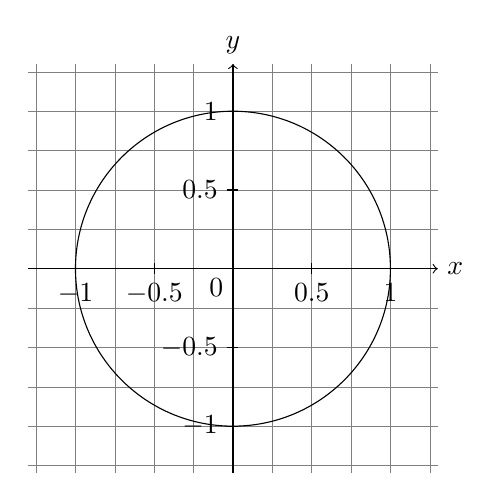
\begin{tikzpicture}[scale=2]
  \draw[help lines, step = 0.25] (-1.3,-1.3) grid (1.3,1.3);
  \draw[->] (-1.3,0) -- (1.3,0) node[right] {$x$};
  \draw[->] (0,-1.3) -- (0,1.3) node[above] {$y$};
  \foreach \x in {-1,-0.5,0.5,1} {\draw (\x,1pt) -- (\x,-1pt) node[below] {$\x$};}
  \foreach \y in {-1,-0.5,0.5,1} {\draw (1pt,\y) -- (-1pt,\y) node[left] {$\y$};}
  \node [below left] at (0,0) {$0$};
  \draw (0,0) circle [radius = 1];
\end{tikzpicture}
\end{frame}

\begin{frame}[label={sec:orge5dea5f}]{Graphing \(\sin(\theta)\) and \(\cos(\theta)\)}
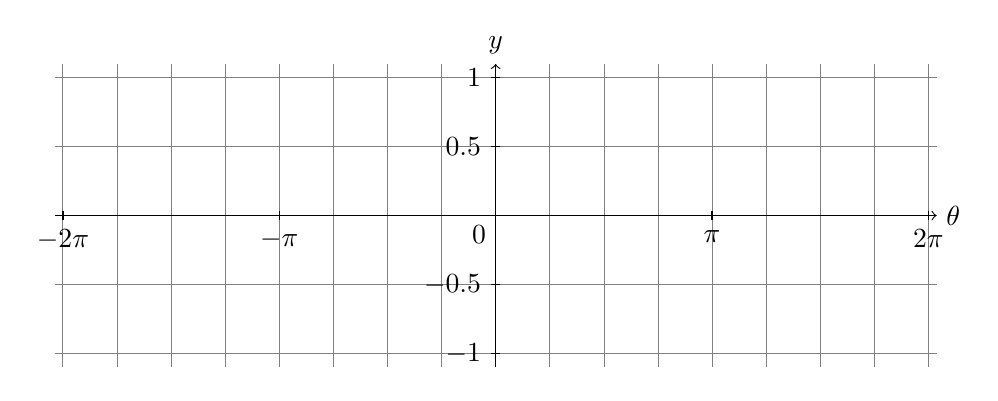
\begin{tikzpicture}
  \begin{scope}[scale=1.75]
  \draw[help lines, xstep = 0.3927, ystep = 0.5] (-3.2,-1.1) grid (3.2,1.1);
  \draw[->] (-3.2,0) -- (3.2,0) node[right] {$\theta$};
  \draw[->] (0,-1.1) -- (0,1.1) node[above] {$y$};
  \foreach \x/\xtext in {-3.14/{-2\pi},-1.57/-\pi,1.57/\pi,3.14/{2\pi}} {\draw (\x,1pt) -- (\x,-1pt) node[below] {$\xtext$};}
  \foreach \y in {-1,-0.5,0.5,1} {\draw (1pt,\y) -- (-1pt,\y) node[left] {$\y$};}
  \node [below left] at (0,0) {$0$};
  \end{scope}
\end{tikzpicture}
\end{frame}

\begin{frame}[label={sec:orga33ecde}]{The Period of \(\sin(\theta)\) and \(\cos(\theta)\)}
We've already discussed the period of \(\sin(\theta)\) and
\(\cos(\theta)\), but let's see if we can determine these from the
graphs we just drew.
\end{frame}

\begin{frame}[label={sec:org3f59487}]{Special Characteristics of Sine and Cosine functions}
The following are special characteristics we can determine from the graphs of \(\sin(\theta)\) and \(\cos(\theta)\):

\begin{enumerate}
\item The domain of both functions is: \uline{\hspace*{1in}}.
\item The range of both functions is: \uline{\hspace*{1in}}.
\item Both functions are periodic with period: \uline{\hspace*{1in}}.
\item \(\sin(\theta)\) is \uline{\hspace*{1in}}, in other words, the graph of \(y = \sin(\theta)\) is symmetric about the origin.
\item \(\cos(\theta)\) is \uline{\hspace*{1in}}, in other words, the graph of \(y = \cos(\theta)\) is symmetric about the y-axis.
\end{enumerate}
\end{frame}

\begin{frame}[label={sec:org2835b6b}]{Investigating General Sinusoidal Functions}
In general, we call any periodic function that oscillates between a
maximum value and a minimum value \uline{\hspace*{1in}}.  Sinusoidal
functions in general can be written as:

\[y = \hspace{1in}\]
or
\[y = \hspace{1in}\]

Let's investigate how all of these numbers affect the shape of the
graph of \(\sin\) and \(\cos\).
\end{frame}

\begin{frame}[label={sec:org2a29113}]{\(A\) (With C and D both 0)}
\end{frame}

\begin{frame}[label={sec:org8dd4c9b}]{Amplitude}
\end{frame}

\begin{frame}[label={sec:orgee14a70}]{\(B\) (With C and D both 0)}
\end{frame}

\begin{frame}[label={sec:org52c1dcd}]{Period}
\end{frame}

\begin{frame}[label={sec:org10d09fc}]{\(C\)}
\end{frame}

\begin{frame}[label={sec:org257121a}]{The Phase Shift}
\end{frame}

\begin{frame}[label={sec:org5349d29}]{\(D\)}
\end{frame}

\begin{frame}[label={sec:org71b181b}]{The Midline}
\end{frame}

\begin{frame}[label={sec:org6c1412c}]{Putting it all together}
So to graph a sinusoidal function \(y = A\sin\left(Bx - C \right) + D\) or \(y = A\cos \left( Bx - C \right) + D\):

\begin{block}{}
\begin{enumerate}
\item Determine the Amplitude: \(\left| A \right|\)
\item Determine the Period: \(\frac{2\pi}{|B|}\)
\item Determine the Phase Shift: \(\frac{C}{B}\)
\item Determine the midline: \(y = D\)
\end{enumerate}
\end{block}
\end{frame}

\begin{frame}[label={sec:org74fc964}]{A Modeling Problem}
Model the number of hours of daylight in Winchester, VA \(t\) days
after January 1 using a sinusoidal function.

\vspace{10in}
\end{frame}
\end{document}